% 2009 年陕西卷文科第 22 题：双曲线 y^2/4 - x^2 = 1、两条渐近线与点 A、B、P。
% 来源 PDF：普通高考/2009/2009陕西文.pdf，SHA-256 c4760285004d01aee97af7821783660b08339cca3a3fc8645052f11001ba586a。
% 原页：第 2 页（A3 三栏）第 3 栏上部，书页码 552。
% 重绘依据：按 y^2/4-x^2=1 与渐近线 y=±2x 等比绘制；取 λ=1/2 的构型
%   A(1.5,3)、B(-0.75,1.5)、P(0.75,2.5)，P 在双曲线上。
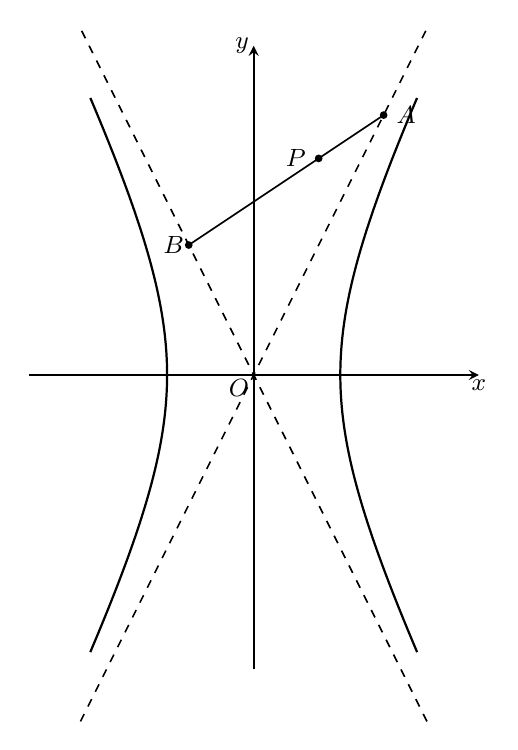
\begin{tikzpicture}[semithick, x=1.1cm, y=1.1cm, every node/.style={inner sep=1.4pt, font=\small}]
  % 坐标轴
  \draw[-stealth] (-2.6,0) -- (2.6,0) node[below] {$x$};
  \draw[-stealth] (0,-3.4) -- (0,3.8) node[left] {$y$};
  \node[below left] at (0,0) {$O$};

  % 渐近线
  \draw[dashed] (-2.0,-4.0) -- (2.0,4.0);
  \draw[dashed] (2.0,-4.0) -- (-2.0,4.0);

  % 双曲线两支
  \draw[domain=-3.2:3.2, samples=160, thick] plot ({sqrt(1+(\x*\x)/4)},{\x});
  \draw[domain=-3.2:3.2, samples=160, thick] plot ({-sqrt(1+(\x*\x)/4)},{\x});

  % 点与直线
  \coordinate (A) at (1.5,3.0);
  \coordinate (B) at (-0.75,1.5);
  \coordinate (P) at (0.75,2.5);
  \fill (A) circle (1.4pt);
  \fill (B) circle (1.4pt);
  \fill (P) circle (1.4pt);
  \draw (A) -- (B);

  % 标注
  \node[right=3pt] at (A) {$A$};
  \node[left] at (B) {$B$};
  \node[left=3pt] at (P) {$P$};
\end{tikzpicture}
